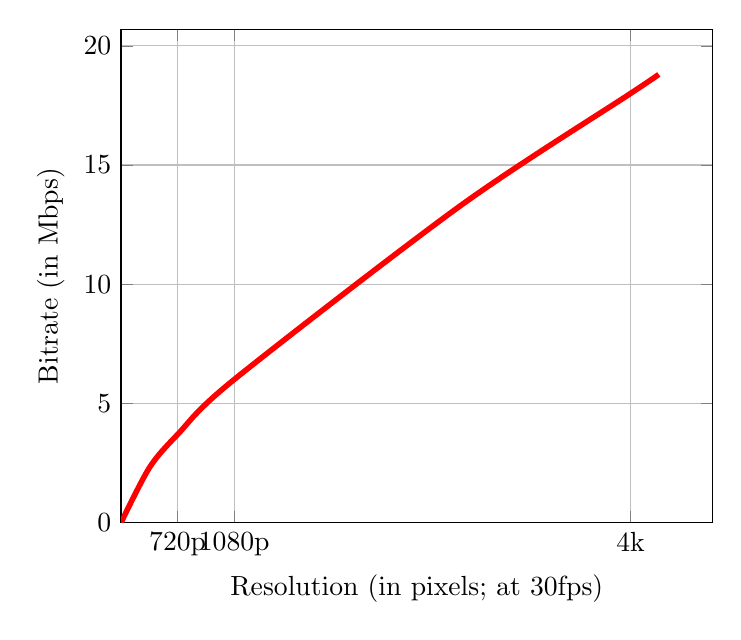
\begin{tikzpicture} %[>=latex]
\begin{axis}[
width=0.75\textwidth,
%line width=2,
%symbolic x coords={2012, 2013, 2014, 2015, 2016},
xtick={2,4,18},
xticklabels={720p,1080p,4k},
%minor xtick={0,1,...,18},
grid=both,
ymin=0,
xmin=0,
xlabel=Resolution (in pixels; at 30fps),
ylabel=Bitrate (in Mbps),
%enlarge x limits=0.1,
%xticklabel style={text width=0.2\textwidth,align=flush left},
]
\addplot[line width=2pt,smooth,color=red] coordinates {
	(0,0)
	(1,2.300)
	(2,3.700)
	%(3,5050)
	(4,6.006)
	(12,13.300)
	(18,18.000)
	(19,18.800)
};
%\draw[red] plot [smooth] coordinates {(0 0) (2,3700) (4,6006) (18,18000)};
\end{axis}
\end{tikzpicture}